\documentclass[10pt]{beamer}
\usetheme[
%%% options passed to the outer theme
%    hidetitle,           % hide the (short) title in the sidebar
%    hideauthor,          % hide the (short) author in the sidebar
%    hideinstitute,       % hide the (short) institute in the bottom of the sidebar
%    shownavsym,          % show the navigation symbols
%    width=2cm,           % width of the sidebar (default is 2 cm)
%    hideothersubsections,% hide all subsections but the subsections in the current section
%    hideallsubsections,  % hide all subsections
%    left                % right of left position of sidebar (default is right)
  ]{Aalborg}
  
% If you want to change the colors of the various elements in the theme, edit and uncomment the following lines
% Change the bar and sidebar colors:
%\setbeamercolor{Aalborg}{fg=red!20,bg=red}
%\setbeamercolor{sidebar}{bg=red!20}
% Change the color of the structural elements:
%\setbeamercolor{structure}{fg=red}
% Change the frame title text color:
%\setbeamercolor{frametitle}{fg=blue}
% Change the normal text color background:
%\setbeamercolor{normal text}{bg=gray!10}
% ... and you can of course change a lot more - see the beamer user manual.

\usepackage[utf8]{inputenc}
%\usepackage[english]{babel}
\usepackage[spanish]{babel}
\usepackage[T1]{fontenc}
\usepackage[demo]{graphicx} 
% Or whatever. Note that the encoding and the font should match. If T1
% does not look nice, try deleting the line with the fontenc.

\usepackage[table,xcdraw]{xcolor}
\usepackage{helvet}
%\usepackage{tikz}
\usetikzlibrary{shapes,arrows,positioning}

%\usepackage{minted}
\usepackage{animate}
\usepackage{media9}
\usepackage[american,symbols]{circuitikz}
\usepackage{amsmath}
\usepackage{amsfonts}
%\usepackage[symbols]{circuitikz}
\ctikzset{v/.append style={/tikz/american voltages}}
\ctikzset {voltage/distance from node=0.7}

\usepackage{listings}
\usepackage{color}
\definecolor{codegreen}{rgb}{0,0.6,0}
\definecolor{codegray}{rgb}{0.5,0.5,0.5}
\definecolor{codepurple}{rgb}{0.58,0,0.82}
\definecolor{backcolour}{rgb}{0.95,0.95,0.92}
 
\lstdefinestyle{mystyle}{
    backgroundcolor=\color{backcolour},   
    commentstyle=\color{codegreen},
    keywordstyle=\color{magenta},
    numberstyle=\tiny\color{codegray},
    stringstyle=\color{codepurple},
    basicstyle=\footnotesize,
    breakatwhitespace=false,         
    breaklines=true,                 
    captionpos=b,                    
    keepspaces=true,                 
    numbers=left,                    
    numbersep=5pt,                  
    showspaces=false,                
    showstringspaces=false,
    showtabs=false,                  
    tabsize=2
}
 
\lstset{style=mystyle}


% colored hyperlinks
\newcommand{\chref}[2]{%
  \href{#1}{{\usebeamercolor[bg]{Aalborg}#2}}%
}

\title[Análisis y Diseño de Circuitos Eléctricos]% optional, use only with long paper titles
{Análisis y Diseño de Circuitos Eléctricos}

\subtitle{Elementos de un circuito}  % could also be a conference name

\date{\today}

\author[Víctor Medrano Zarazúa] % optional, use only with lots of authors
{
  Víctor Medrano Zarazúa\\
  \href{mailto:victor_medrano@my.uvm.edu.mx}{{\tt victor\_medrano@my.uvm.edu.mx}}
}
% - Give the names in the same order as they appear in the paper.
% - Use the \inst{?} command only if the authors have different
%   affiliation. See the beamer manual for an example

\institute[
%  {\includegraphics[scale=0.2]{aau_segl}}\\ %insert a company, department or university logo
  %Dept.\ of Electronic Systems\\
  Universidad del Valle de México\\
  Campus Monterrey
] % optional - is placed in the bottom of the sidebar on every slide
{% is placed on the bottom of the title page
  %Department of Electronic Systems\\
  Universidad del Valle de México\\
  Campus Monterrey
  %Universidad Autónoma de Nuevo León\\
  %Facultad de Ingeniería Mecánica y Eléctrica
  
  %there must be an empty line above this line - otherwise some unwanted space is added between the university and the country (I do not know why;( )
}

% specify the logo in the top right/left of the slide
\pgfdeclareimage[height=1cm]{mainlogo}{AAUgraphics/UVM} % placed in the upper left/right corner
\logo{\pgfuseimage{mainlogo}}

% specify a logo on the titlepage (you can specify additional logos an include them in 
% institute command below
\pgfdeclareimage[height=1.5cm]{titlepagelogo}{AAUgraphics/UVM} % placed on the title page
%\pgfdeclareimage[height=1.5cm]{titlepagelogo2}{AAUgraphics/aau_logo_new} % placed on the title page
\titlegraphic{% is placed on the bottom of the title page
  \pgfuseimage{titlepagelogo}
%  \hspace{1cm}\pgfuseimage{titlepagelogo2}
}

%\definecolor{UniBlue}{RGB}{255,255,255}

\tikzset{
block/.style={
  draw, 
  fill=blue!20, 
  rectangle, 
  minimum height=3em, 
  minimum width=6em
  },
 gain/.style={
    draw,
    fill=blue!20, 
    isosceles triangle,
    minimum height = 3em,
    isosceles triangle apex angle=60
    },
sum/.style={
  draw, 
  fill=blue!20, 
  circle, 
  },
input/.style={coordinate},
output/.style={coordinate},
pinstyle/.style={
  pin edge={to-,thin,black}
  }
}  

\begin{document}
% the titlepage


%\setbeamercolor{title}{fg=UniBlue}
%\setbeamercolor{normal text}{fg=UniBlue}
%\setbeamercolor{Aalborg}{fg=black,bg=black}


{\aauwavesbg
\begin{frame}[plain,noframenumbering] % the plain option removes the sidebar and header from the title page
  \titlepage
\end{frame}}
%%%%%%%%%%%%%%%%

% TOC
\begin{frame}{Contenido}{}
\tableofcontents
\end{frame}
%%%%%%%%%%%%%%%%
\section{Repaso}

\begin{frame}{Repaso}{}
\begin{block}{Recapítulemos...}
\begin{itemize}
\item ¿Qué es un \href{https://www.youtube.com/watch?v=97CWXZa66C4} {\textcolor{blue}{Googol}?}
\item ¿Cuál es la diferencia entre notación científica y notación de ingeniería?
\item ¿Qué prefijos utilizamos en la notación de ingeniería y que origen tienen?
\end{itemize}
\end{block}

\end{frame}

\section{Introducción}
%\section{Carga eléctrica}
\begin{frame}{Introducción}{}

\begin{block}{Análisis y diseño}
\begin{itemize}
    \item Para poder analizar y diseñar circuitos necesitamos elementos con los cuales construir circuitos
    \item Presentaremos los elementos esenciales en la construcción de circuitos.
\end{itemize}
\end{block}

\end{frame}

\section{Componentes ideales}
\begin{frame}{Componentes ideales de un circuito}{Elementos pasivos}
\begin{block}{Componentes ideales básicos}
\begin{itemize}
    \bigskip
    \item Resistencia ($\mathnormal{R}$)
    \begin{figure}[h!]
    \begin{circuitikz}[/tikz/circuitikz/bipoles/length=0.8cm, scale=0.1,american voltages,D*, v^>=$\mathnormal{v}$,i>_=$\mathnormal{i}$] \draw
        (0,5) to[resistor] (20,5)
    ;  
    \end{circuitikz}
    \end{figure}
    \item Capacitor ($\mathnormal{C}$)
    \begin{figure}[h!]
    \begin{circuitikz}[/tikz/circuitikz/bipoles/length=0.8cm, scale=0.1,american voltages,D*, v^>=$\mathnormal{v}$,i>_=$\mathnormal{i}$] \draw
        (0,5) to[capacitor] (20,5)
    ;  
    \end{circuitikz}
    \end{figure}
    \item Inductor ($\mathnormal{L}$)
    \begin{figure}[h!]
    \begin{circuitikz}[/tikz/circuitikz/bipoles/length=0.8cm, scale=0.1,american voltages,D*, v^>=$\mathnormal{v}$,i>_=$\mathnormal{i}$] \draw
        (0,5) to[inductor] (20,5)
    ;  
    \end{circuitikz}
    \end{figure}
\end{itemize}
\end{block}
\end{frame}

\begin{frame}{Componentes ideales de un circuito}{Elementos pasivos}
\begin{block}{Ecuaciones I-V}
La relación corriente-voltaje en cada elemento ideal de un circuito (resistencia, capacitor e inductor respectivamente) es definido por la siguientes ecuaciones.
\end{block}
\begin{equation}
    \mathnormal{v = iR}
    \label{eqn:ohmslaw}
\end{equation}
\begin{equation}
    \mathnormal{i = C \frac{dv}{dt}}
\end{equation}
\begin{equation}
    \mathnormal{v = L \frac{di}{dt}}
\end{equation}

La ecuación \ref{eqn:ohmslaw} también es llamada Ley de Ohm. Y la usaremos una y otra vez en este curso.

\end{frame}

\section{Fuentes ideales}

\begin{frame}{Fuentes ideales}{Elementos activos}
\begin{block}{Tipos de fuentes ideales}
Existen dos tipos de fuentes ideales:
\medskip
\begin{itemize}
    \item Fuente ideal de voltaje: Entrega un voltaje constante
    \begin{columns}[c]
    \column{0.8in}
    \begin{figure}[h!]
    \begin{circuitikz}[/tikz/circuitikz/bipoles/length=1cm, scale=0.1,american voltages] \draw
        (0,5) to[american voltage source] (20,5)
    ;  
    \end{circuitikz}
    \end{figure}
    \column{0.8in}
    \begin{figure}[h!]
    \begin{circuitikz}[/tikz/circuitikz/bipoles/length=1cm, scale=0.1,american voltages] \draw
        (0,5) to[battery] (20,5)
    ;  
    \end{circuitikz}
    \end{figure}
    \column{0.8in}
    \begin{figure}[h!]
    \begin{circuitikz}[/tikz/circuitikz/bipoles/length=1cm, scale=0.1,american voltages] \draw
        (0,5) to[battery1] (20,5)
    ;  
    \end{circuitikz}
    \end{figure}
    \end{columns}
    
    \medskip
    
    \item Fuente ideal de corriente: Entrega una corriente constante
    \begin{columns}[c]
    \column{0.8in}
    \begin{figure}[h!]
    \begin{circuitikz}[/tikz/circuitikz/bipoles/length=1cm, scale=0.1,american voltages] \draw
        (0,5) to[american current source, invert] (20,5)
    ;  
    \end{circuitikz}
    \end{figure}
    \column{0.8in}
    \begin{figure}[h!]
    \begin{circuitikz}[/tikz/circuitikz/bipoles/length=1cm, scale=0.1,american voltages] \draw
        (0,5) to[american current source] (20,5)
    ;  
    \end{circuitikz}
    \end{figure}
    \end{columns}
\end{itemize}
\medskip
Estos elementos entregarán potencia a nuestro circuito.
\end{block}
\end{frame}

\begin{frame}{Fuentes ideales}{Elementos activos}
\begin{block}{Curvas características}
Las fuentes de voltaje y corriente ideales poseen las siguientes curvas características.

\end{block}
\begin{columns}[c]
    \column{1.2in}
\begin{figure}[h!]
\centering
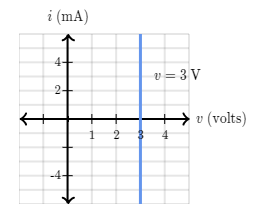
\includegraphics [scale=0.6]{constvolt}
\label{fig:first}
\end{figure}

    \column{1.2in}
\begin{figure}[h!]
\centering
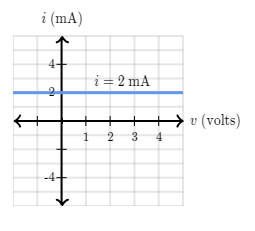
\includegraphics [scale=0.6]{constcurr}
\label{fig:first}
\end{figure}
\end{columns}

\end{frame}

%%%%%%%%%%%%%%%%%%%%%%%%%%%%5
\section{Información de contacto}
% contact information
\begin{frame}{Feedback}{Información de contacto}
En caso de comentarios, sugerencias, preguntas o errores en las diapositivas no dudes en contactarme.
  \begin{center}
    \insertauthor\\
    \chref{https://mixlaab.github.io}{https://mixlaab.github.io}\\
    WA: 8119022700\\
    %9220 Aalborg Ø
  \end{center}
\end{frame}
%%%%%%%%%%%%%%%%

{\aauwavesbg%
\begin{frame}[plain,noframenumbering]%
  \finalpage{Fin}
\end{frame}}
%%%%%%%%%%%%%%%%

\end{document}
